{ %section3_5
	\subsection{Ошибки в многопоточных приложениях}
	\parПомимо привычных для программиста ошибок, встречающихся в компьютерных программах, существует ряд ошибок, специфичных для параллельного программирования. Эти ошибки обусловлены следующими особенностями параллельных программ: 
	\begin{itemize}
		\item\textbf{Синхронизация потоков.} Программист должен обеспечить корректную последовательность выполняемых разными потоками операций. В общем случае невозможно точно сказать, в какой последовательности будут выполняться команды потоков, т.к. операционная система может в произвольный момент времени при остановить выполнение потока.
		\item\textbf{Взаимодействие потоков.} Также программист не должен конфликтов при обращении к общим для потоков областям памяти. 
		\item\textbf{Балансировка нагрузки.} Если в распараллеленной программе один из потоков выполняет 99\% работы, то даже на 64-ядерной системе параллельное ускорение едва ли превысит значение 1.01.
		\item\textbf{Масштабируемость.} В идеале параллельная программа должна одинаково хорошо распараллеливать выполняемую работу на любом доступном количестве процессоров. Однако добиться этого нелегко и это часто приводит к трудно обнаруживаемым ошибкам.
	\end{itemize}
	\parРассмотрим далее подробнее следующий неполный перечень типовых ошибок, возникающих в параллельных программах независимо от используемой технологии распараллеливания:
	\begin{itemize}
		\itemПотеря точности операций с плавающей точкой.
		\itemВзаимные блокировки (deadlock).
		\itemСостояния гонки (race conditions). 
		\itemПроблема АВА.
		\itemИнверсия приоритетов.
	\end{itemize}
	\par\textbf{Потеря точности.} Если параллельная программа используется для проведения операций с плавающей точкой при работе с вещественными  переменными, расположенными в общей для потоков памяти, то при каждом запуске программы может получаться разный результат вещественных расчётов. Это объясняется тем, что при работе нескольких потоков невозможно точно предсказать, в каком порядке операционная система предоставит этим потокам процессор, т.к. в любой момент любой поток может быть временно приостановлен по усмотрению ОС. Это в свою очередь приводит к неопределённой последовательности выполнения операций с плавающей точкой, результат которых, как известно, может зависеть от порядка.
	\parРассмотрим пример, иллюстрирующий сказанное:
	\begin{figure}[H]
		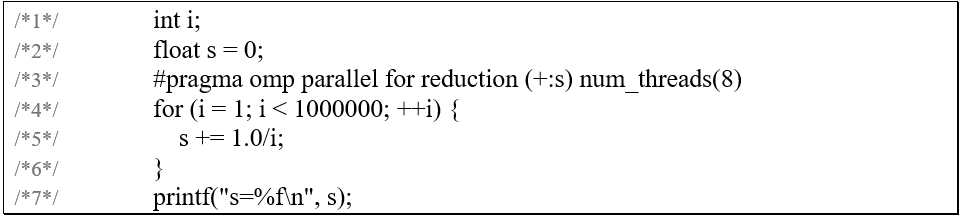
\includegraphics[width=1\linewidth]{OpenMPExample16}
	\end{figure}
	\parЗдесь в переменную s суммируются результаты вещественных вычислений восемью потоками. В результат получается s=14.393189. Однако если эту же программу выполняет всего один поток (для этого нужно в строке 3 установить значение параметра num\textunderscore threads в 1), то результат получится иным: s=14.357357. Различие между двумя приведёнными значениями составляет примерно 0.25\%. 
	\parПолучается, что параллельная программа может давать разный результат при запуске на разных платформах. Это следует учитывать, проводя верификацию параллельных программ с использованием однопоточных их нераспараллеленных аналогов.
	\par\textbf{Взаимные блокировки.} Одним из часто используемых примитивов синхронизации является мьютекс, позволяющий нескольким потокам согласованно и последовательно выполнять критические области кода, расположенные внутри параллельных секций кода. Критические секции замедляют работу программы, т.к. в каждый момент времени только один поток может находиться внутри критической секции. С помощью мьютексов, например, реализуются функции omp\textunderscore set\textunderscore lock и omp\textunderscore unset\textunderscore lock в OpenMP. При обрамлении этими функциями некоторого участка кода можно сделать из него критическую секцию, вход в которую контролируется условным программным замком (lock). В сложных программах может использовать несколько замков. Это может привести к тому, что два потока, захватывающие несколько замков, застопорят выполнение друг друга без всякой возможности выйти из состояния ожидание друг друга. Такая ситуация называется deadlock (взаимная блокировка).
	\par Простейшим примером взаимной блокировки является работа двух потоков, первый из которых захватывает сначала замок1, потом замок2, а второй сначала захватывает замок2, потом замок 1. В результате, возникнет deadlock, если операции будут выполняться в следующем порядке: 
	\begin{itemize}
		\itemпоток1 захватил замок1;
		\itemпоток2 захватил замок2;
		\itemпоток1 бесконечно ждёт освобождения замка 2;
		\itemпоток2 бесконечно ждёт освобождения замка 1.
	\end{itemize}
	\parОдна из неприятных сторон описанной ситуации заключается в том, что далеко не всегда взаимная блокировка происходит при отладке программы, когда её можно было бы легко выявить и исправить, т.к. вероятность наложение событий нужным образом может быть очень мала. В результате работающая и сданная заказчику программа может в случайные моменты времени "зависать"\verb+ +по якобы непонятным причинам. Рассмотрим пример искусственно реализованной взаимоблокировки, в котором можно рассчитать вероятность её возникновения при многократном запуске.
	\parВ приведённой ниже программе в строке 7 создаётся поток, который в бесконечном цикле захватывает замок1, замок2 и инкрементирует переменную s, освобождая после этого оба замка. В строке 13 создаётся поток, которой тоже бесконечно инкрементирует s, однако захватывает замки в другом порядке: замок2, замок1. В строке 19 создаётся поток, который следит за состоянием s, опрашивая эту переменную каждые 10 мс. Если последний поток обнаруживает, что переменная s перестала изменяться, он печатает сообщение о возникшей взаимоблокировке и завершает программу.  
	\begin{figure}[H]
		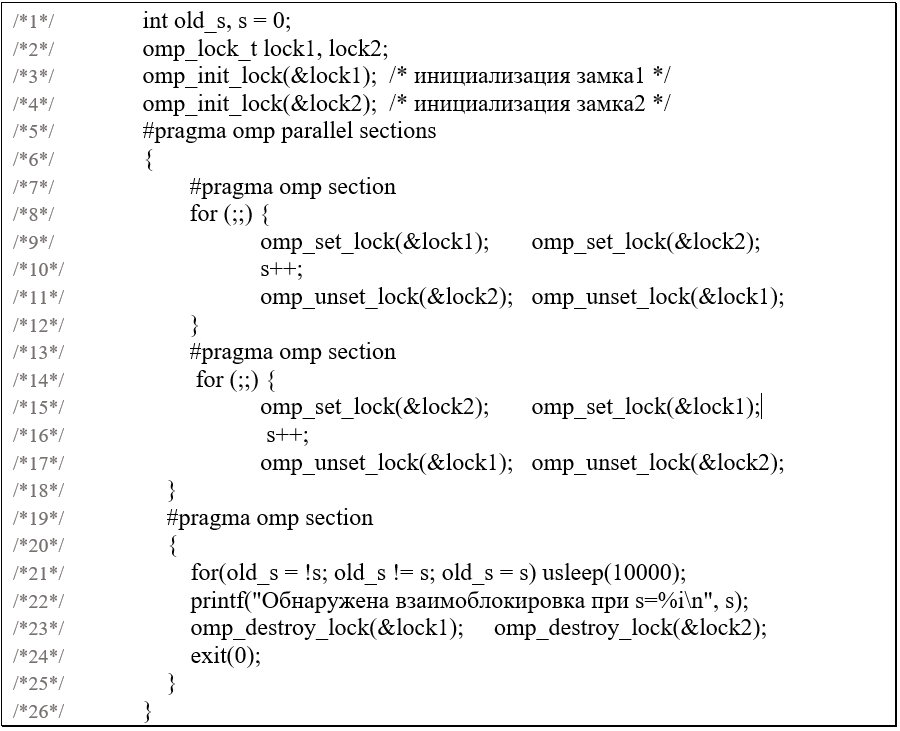
\includegraphics[width=1\linewidth]{deadlockExample}
	\end{figure}
	\parЭксперименты с приведённой программой проводились на компьютере с процессором Intel Core i5 (4 логических процессора) с 8 гигабайт ОЗУ в операционной системе Debian Wheezy. Программы была запущена 10000 раз, и было получено 10000 значений переменной s на момент возникновения взаимоблокировки. Результаты этих измерения приведены на рисунке~\ref{GraphDeadlock:image} в виде гистограммы плотности распределения s.
	\parНа приведённом рисунке на оси абсцисс подписаны правые границы столбиков. Последний столбик содержит все попадания от 3000 до бесконечности. Среднее значение s в описанном случае оказалось равным 2445, т.е. два потока успевают примерно 1222.5 раза захватить и отпустить замки в заведомо неверном опасном порядке без возникновения взаимоблокировки.
	\begin{figure}[H]
		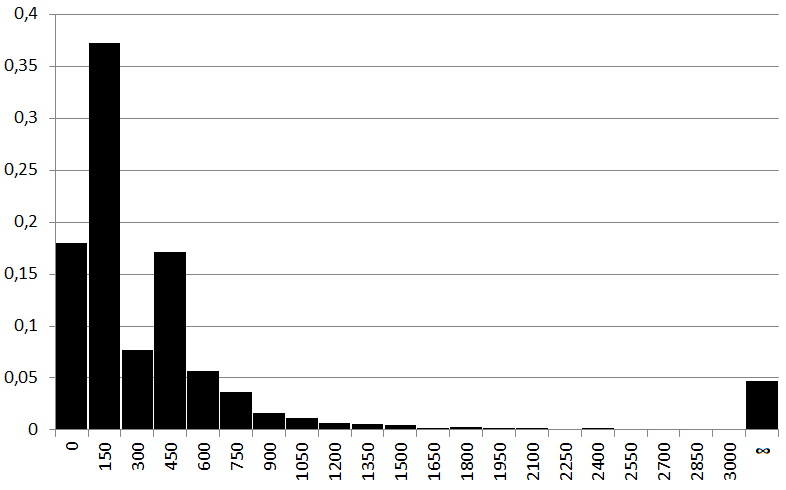
\includegraphics[width=1\linewidth]{GraphDeadlock}
		\caption{\textit{Гистограмма распределения количества запусков параллельной программ до возникновения взаимоблокировки}}
		\label{GraphDeadlock:image}
	\end{figure}
	\parДля исправления описанной ошибки нужно сделать порядок захвата замков одинаковым во всех потоках. Иногда советуют во всей программе установить некоторое общее правило захвата замков, например, можно захватывать замки в алфавитном порядке.
	\parПомимо описанной ситуации с неверным порядком захвата мьютексов, существуют и другие причины взаимоблокировок. Например, повторный захват мьютекса (замка). Неверно написанная программа может попытаться повторно захватить уже захваченный ею замок, предварительно его не освободив. При этом повторная попытка захвата полностью останавливает работу потока. Если логика программы требует повторный захват мьютекса (например, для организации рекурсии), следует использовать специальный подвид замков: рекурсивные мьютексы.
	\par
}